\chapter{端到端语音识别汇总}
%------------------------------------------------------------------------------
%                                CTC 
%------------------------------------------------------------------------------
\section{CTC}
\label{sec:ctc}
CTC说实话,就是比较麻烦……我已经看过很多遍了,不过看的原理居多,代码这块,前后向的实现以及梯度的求取这些都没看过……先总结下CTC的基本原理吧还是。

列出本节参考的一些文献和博客:
\begin{enumerate}
  \item CTC的开山之作\upcite{Graves_ctc}\href{http://www.cs.toronto.edu/~graves/icml_2006.pdf}{《Connectionist Temporal Classification: Labelling Unsegmented Sequence Data with Recurrent Neural Networks》},不建议看这篇……因为这篇在讲到求输出序列的时候使用的前后向算法中前向和后向算法的时候对当前时刻$t$的输出概率算了两遍,后面还得再去掉,感觉没啥意思。其次在介绍前后向算法的时候不够简洁,比他的博士论文复杂不少;
  \item Graves大佬的博士毕业论文\upcite{Graves_thesis}\href{https://www.cs.toronto.edu/~graves/preprint.pdf}{《Supervised Sequence Labelling with Recurrent Neural Networks》}里面的推导过程写的就相对来说更清楚一些,过程非常简洁,虽然还有一点点小错误,但是不影响整体的理解,所以推荐看这个来搞清楚CTC的前世今生;
  \item 关于CTC的原理图形化描述请参考\href{https://distill.pub/2017/ctc/}{sequence modeling with ctc\upcite{ctc_graph}},用很多小例子来展现CTC的原理和解码等,有助于去理解结果;
  \item 关于CTC求导部分\upcite{ctc_grad}的得到最后一步结果可以参考\href{https://blog.csdn.net/w5688414/article/details/77867786}{教程:Connectionist Temporal Classification详解补充};
  \item 关于CTC前后向python代码实现请参考\href{https://blog.csdn.net/JackyTintin/article/details/79425866}{CTC 原理及实现}。
\end{enumerate}

以上资料看完,我觉得就完全可以理解CTC的原理了,当然手推公式是少不了的,接下来进入正题。
\subsection{白话CTC}
首先明确:语音识别是一个序列分类的任务,那么其输入是逐帧的,如果不知道每一帧对应的标签,那么我们想要用 connectionist network 去干这件事,就得有目标函数。整个神经网络学习的准则就来自于目标函数,所以什么都可以没有,不能没有目标函数;话又说回来了,语音识别在训练的时候,逐帧输入,则必然对应着逐帧的输出,如果不想要对齐,想要端到端,那么就必须想办法把这些逐帧的输出映射成序列输出。真正难的地方就在这儿,怎么去映射,映射了之后怎么定义目标函数;

CTC就是来干这个事情的。

我们先回忆一下使用传统的HMM-DNN模型来搭建语音识别框架,其中包含很多个子任务。首先我们需要使用EM算法训练HMM-GMM模型以拿到对齐的数据,即一帧对应一个音素。其次以这些数据来训练DNN模型,训练好了DNN模型之后,通过HMM和vocabulary映射到更高的建模单元,再结合词典、语言模型来用WFST进行解码。

好的,这个过程很复杂,而且每一块信息量都很足,即要花很多的精力去学习和设计;

不用担心,现在端到端已经越来越火热,效果看上去也是越来越好了。那么咱们说一说CTC是怎么干的。

CTC呢,有一些很重要的设定:\textcolor{red}{(1)每一帧的输出是相互独立的;(2)只要最终映射出来的序列是对的,在任何时刻输出某个标签都可以。}有个图很好玩,来自PilgrimHui的博客\upcite{ctc_free},如图\ref{fig:ctc-free}。我觉得这个图很好的说明了CTC的内涵和特点。
\begin{figure}[h]
  \centering
  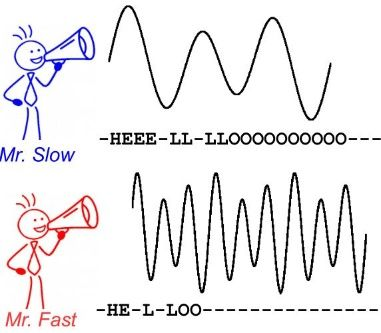
\includegraphics[width=0.7\textwidth]{ctc_free}
  \caption{同一单词不一样的输出音频的图解 \label{fig:ctc-free}}
\end{figure}

第一个设定是为了后面使用最大似然估计去定义loss函数的,第二个设定呢就是彻底扔掉对齐数据的限制,按照这个设定,是没有固定的对齐结果的。在讲怎么从连续帧的输出映射到一整个序列之前,我们还要再讲一讲一些规则。为了\textcolor{blue}{避免相邻输出相同和更好的对建模单元的边界进行建模},CTC引入了一个非常重要的输出标签:blank。你可以认为这个东西就是没有标签的意思,因为它的出现对句中无意义的片段比如静音段提供了建模单元。

假设字母表为$A$,则$A^{'}=A\cup\{blank\}$,激活函数的输出$y_k^{t}$为$t$时刻输出$A^{'}$中元素$k$的概率值,给定输入长度为$T$的音频序列$x$;基于输出标签集合$A^{'}$,定义$A^{'^{T}}$为长度为$T$的序列集合。

CTC有如下假设:\textcolor{red}{每一个时间步输出的标签概率值与其他时间步之间相互独立,或者说在$x$的条件下,相互独立}。

那么对于$\pi\in{A^{'^{T}}}$,其条件概率如公式\ref{eqn:ctc-pi}。
\begin{align}
\label{eqn:ctc-pi}
  P(\pi|x) = \prod_{t=1}^{T}y_{\pi_{t}}^{t}
\end{align}

为了和域$A$内的标签序列$l$区分开来,我们称$\pi$为域$A^{'}$内的一条路径。由此定义一个 many-to-one 的函数:$\mathcal{F}:A^{'^{T}}\mapsto{A^{\leq{T}}}$,因为最终系统要输出的是整个正常的序列,而不是穿插着一堆blank还有一堆重复label的奇奇怪怪的东西,我们得到的$\pi$是沿着时间线严格输出的标签值,而$l$是实际上某句话的内容,所以需要$\mathcal{F}$来映射成我们需要的结果,这样才能叫做端到端呀。举个例子,比如某一段音频有15帧,这15帧说的是英文单词"beef",这个就是$l$,那实际上有15帧就会输出15帧的输出结果,可能是这样的"\_ \_ b b \_ e \_ \_ e e \_ f f \_ \_",这个就是$\pi$,$\mathcal{F}$干的事就是把$\pi$映射成$l$,其规则是:
\begin{enumerate}
  \item 合并重复的标签:"\_ \_ b b \_ e \_ \_ e e \_ f f \_ \_" $\longrightarrow$ "\_ b \_ e \_ e \_ f \_";
  \item 移除blank:"\_ b \_ e \_ e \_ f \_" $\longrightarrow$ "beef"。
\end{enumerate}}

这样的路径有很多很多条,而每一条路径都是排他的,因此我们就可以通过公式\ref{eqn:ctc-p}计算出域$A$内某个标签序列的概率值了,即从一段音频中,输出一句话的概率值,CTC牛逼。
\begin{align}
\label{eqn:ctc-p}
  P(l|x) = \sum_{\pi\in{\mathcal{F}^{-1}(l)}}P(\pi|x)
\end{align}

这种整合的意义在于 我不在乎你在什么时间点输出什么,我只在乎最后映射的结果是我想要的。只要最终结果是一样的,中间有多少个blank,同样的标签重复了多少次,我不在乎。这就使得CTC可以使用没有对齐的数据来进行语音识别。

好的,现在还剩下一些问题,公式\ref{eqn:ctc-p}这玩意怎么计算,穷举吗?计算机表示:无能为力。序列越长,标签越多,尤其是碰到汉语这种用字建模的,基本上想都不要想。回想起HMM中讲到的前后向算法,CTC也可以这么干啊,毕竟都是路径概率求解问题。

\subsection{CTC中的前后向算法}
对于公式\ref{eqn:ctc-p},假设标签序列的长度为$U$,音频的长度为$T$,共有$2^{T-U^{2}+U(T-3)}3^{^{(U-1)(T-U)-2}}$条路径。

………………

说实话,我不知道这个是怎么算出来的,但是还是挺恐怖的,还是按照上面举的例子,$U=4$,$T=15$,算一下就是$2^{47}3^{31}$。

………………

再见!

前后向算法的核心是标签序列$l$对应的所有路径概率和可以转换成标签前缀的迭代求和。

为了能让blank出现在输出路径中,我们将$l$修改下,在$l$的前后都加上blank,同时在每个标签之间也都加上blank,记作 $l^{'}$即"b e e f"$\longrightarrow$"\_ b \_ e \_ e \_ f \_"。若$l$的长度为$U$,则$l^{'}$的长度为$U^{'}=2U+1$。为计算$l^{'}$的前缀概率,我们允许blank和non-blank、非重复的non-blank之间直接转换,多解释下这句话的意思:"beef"这个词,"b"在下一个时刻直接跳转到"b"、"e"或者"\_"都是可以的,但是第一个"e"只能跳转到自己本身"e"和"\_",不可以跳转到下一个"e",不然的话,在进行合并操作的时候,第二个"e"就没了,这个需要好好理解,因为后面的前后向算法里面有用到这个特点。

对于一个标签序列$l$,前向变量$\alpha(t,u)$表示所有长度为$t$的路径的概率和,这些路径通过$\mathcal{F}$映射到$l$中长度为$u/2$的前缀,$u/2$向下取整。对于序列$s$,$s_{p:q}$为$s$的子序列${s_p, s_{p+1}, ..., s_{q-1}, s_q}$,定义集合$V(t,u)=\{\pi\in{A^{'^{t}}}:\mathcal{F}(\pi)=l_{1:{u/2}}, \pi_{t}=l_{u}^{'}\}$,则$\alpha(t,u)$的计算如公式\ref{eqn:ctc-forward}。
\begin{align}
\label{eqn:ctc-forward}
  \alpha(t,u) = \sum_{\pi\in{V(t,u)}} \prod_{i=1}^{t}y_{\pi_i}^{i}
\end{align}

我们可以通过$t-1$时刻的前缀来计算$\alpha(t,u)$。

给定上面的公式,我们就可以求得$l$的概率,其等于$T$时刻标签为blank和non-blank的前向概率和,如公式\ref{eqn:ctc-forward-all}。
\begin{align}
\label{eqn:ctc-forward-all}
  p(l|x) = \alpha(T, U^{'}) + \alpha(T, U^{'}-1) 
\end{align}

所有正确的路径一定是以blank或者$l$中的第一个元素开头的,因此我们可以得到$\alpha(t,u)$的初始值,如公式\ref{eqn:ctc-forward-init}。
\begin{align}
\label{eqn:ctc-forward-init}
  \begin{split}
    \alpha(1,1) &= y_{b}^1  \\
    \alpha(1,2) &= y_{l_{1}}^1 \\
    \alpha(1,u) &= 0, \forall u > 2
  \end{split}
\end{align}

初始化的值得到之后,我们可以通过对前缀进行迭代求和的方式得到当前时刻标签索引为$u$的路径概率值,如公式\ref{eqn:ctc-forward-t}。
\begin{align}
\label{eqn:ctc-forward-t}
  \alpha(t,u) = y_{l_{u}^{'}}^{t}\sum_{i=f(u)}^{u} \alpha(t-1,i) 
\end{align}
其中$f(u)$如公式\ref{eqn:ctc-forward-t-start}。
\begin{equation}
\label{eqn:ctc-forward-t-start}
f(u)=\left\{
\begin{array}{rcl}
u-1 & & l_u^{'}=l_{u-2}^{'}\\
u-2 & & otherwise\\
\end{array} \right.
\end{equation}

我觉得有必要解释下公式\ref{eqn:ctc-forward-t-start}。

公式\ref{eqn:ctc-forward-t}左边表示的是在$t$时刻标签索引为$u$的输出概率,右边是在已经确定了$t$时刻输出索引为$u$的情况下,$t-1$时刻的前向概率。因为已经确定了$t$时刻的输出,因此我们需要知道在$t-1$时刻,哪些标签能够在下一个时刻转移到标签$u$。对这些可能的标签前向概率求和,再乘以当前时刻的概率,就得到了我们想要的$\alpha(t,u)$。

那么$t-1$时刻究竟可能是哪些标签呢?

我们还是拿"beef"举例子。

$l=$"b e e f",$l^{'}=$"\_ b \_ e \_ e \_ f \_",为了说的更清楚,我们来给$l^{'}$里面的字母都来标个号,$l^{'}=$"\_(1) b(2) \_(3) e(4) \_(5) e(6) \_(7) f(8) \_(9)"先来看第一种情况,如果$t$时刻的标签$u$有$l_u^{'}=l_{u-2}^{'}$,那么$l_{u}^{'}=$"e(6)"或者$l_{u}^{'}=$"\_(i)",i=\{3,5,7,9\}。
\begin{enumerate}
  \item $l_{u}^{'}=$"e(6)":那么$t-1$时刻的标签等于"e(6)"是完全有可能的;等于\_(5)也是完全可以的;那么能等于e(4)可以吗?假设可以,连起来看$t-1$和$t$时刻的子序列,就是"e(4)e(6)",乍一看好像没问题啊,但是要知道我们在训练的时候"e"是标签,是没有"e(4)"和"e(6)"这种形式的标签的,他们都是"e",根据上面说的CTC的合并规则,这俩就会合并成一个,无法表征两个相同的连续元素。也就是说,CTC是不允许两个相同的连续元素直接跳转过去的,"e(4)"是不可以直接跳转到"e(6)",所以啊,$f(u)=u-1$表示前一个时刻的标签索引只可能和当前时刻的索引相同或者是当前时刻的索引的前一个;
  \item $l_{u}^{'}=$"\_(i)",i=\{3,5,7,9\}:这个解释起来和上面是一样一样的。同样我们的输出标签里面就只有"\_"这个东西,所以按照合并规则,但凡重复了的"\_"都看作是同一个"\_",因此是没有办法表征序列$l^{'}$中的上一个"\_",因此$f(u)=u-1$。
\end{enumerate}

当$l_u^{'} \ne l_{u-2}^{'}$,这个就比较无所谓了,咱们举个例子,假设$l_{u}^{'}=$"f(8)",同样$t-1$时刻的输出为"f(8)"没得问题,"\_(7)"也没得问题,"e(6)"当然也没得问题,反正他们不会乱合并。所以有$f(u)=u-2$。

对应$t$时刻的$u$不能太小,太大无所谓大,大不了剩下的$T-t$帧都重复输出某一个标签或者blank就可以了。如果太小,剩下的$T-t$帧的输出都不够剩下还没有输出的标签了,所以考虑最极端的一种情况就是剩下的每一帧都输出一个$l$中的标签,且这些标签不会自身重复,也就是说每一帧输出的标签都只会输出一次,这样刚好够完整的输出$l$。这就是临界条件,因此我们可以得到$u$的取值范围:
\begin{align}
  T-t \ge \frac{U^{'}-u-1}{2}
\end{align}
解得:
\begin{align}
  u \ge U^{'}-2(T-t) - 1
\end{align}
反过来说,也就是意味着:
\begin{align}
  \alpha(t,u) &= 0, \forall u < U^{'}-2(T-t) - 1
\end{align}

前向算法讲完了,后向算法就很类似了。同样我们定义一个后向变量$\beta(t,u)$,如果说想要得到输出序列$l$,假定$t$时刻的输出是$l_{u}^{'}$,$\beta(t,u)$可以看成是这一些路径的后部分,我们定义$\beta(t,u)$为$t+1$时刻配合上$\alpha(t,u)$恰好构成完整的$l$的所有的后缀路径的概率总和。比照着$V(t,u)$,定义集合$W(t,u)=\{\pi\in{A^{'^{T-t}}:\mathcal{F}(\hat{\pi}+\pi)=l,\forall{\hat{\pi}}\in{V(t,u)}\}$。那么直接计算$\beta(t,u)$的公式如\ref{eqn:ctc-backward}。
\begin{align}
\label{eqn:ctc-backward}
  \beta(t,u) = \sum_{\pi\in{W(t,u)}} \prod_{i=1}^{T-t}y_{\pi_i}^{t+i}
\end{align}

后向算法的初始化如公式\ref{eqn:ctc-backward-init}。
\begin{align}
\label{eqn:ctc-backward-init}
  \begin{split}
    \beta(T,U^{'}) &= 1  \\
    \beta(T,U^{'}-1) &= 1 \\
    \beta(T,u) &= 0, \forall u < U^{'}-1 \\
    \beta(T,U^{'}+1) &= 0
  \end{split}
\end{align}

公式\ref{eqn:ctc-backward-t}描述了$\beta(t,u)$的计算方式。
\begin{align}
\label{eqn:ctc-backward-t}
  \beta(t,u) = \sum_{i=u}^{g(u)} \beta(t+1,i) y_{l_{i}^{'}}^{t+1}
\end{align}
其中:
\begin{equation}
\label{eqn:ctc-backward-t-start}
g(u)=\left\{
\begin{array}{rcl}
u+1 & & l_u^{'}=l_{u+2}^{'}\\
u+2 & & otherwise\\
\end{array} \right.
\end{equation}

公式\ref{eqn:ctc-backward-t-start}表明了对$t+1$时刻能达到的标签的限制,这部分和前向很类似,在此就不再赘述了。

同样后向算法中的$u$不能太大,因为$u$过大的意思就是前$t$个时刻得输出$u$个标签,如果说$t$稍微小了点,那就不够输出这么多标签了。同样,考虑临界条件:前$t$个时刻恰好能够无重复的输出non-blank标签。我们就可以得到如下不等式:
\begin{align}
  t \ge \frac{u}{2}
\end{align}
解得:
\begin{align}
  u \leq 2t
\end{align}
即:
\begin{align}
  \beta(t,u) &= 0, \forall u > 2t
\end{align}

上述迭代过程,中间会涉及到概率的求和,如果直接就在计算机中按照上述方式实现的话,很容易就会导致underflows,所以需要将概率变成$\log$概率值,对于两个概率的和,我们一般使用公式\ref{eqn:log-scale}来实现,等到算完之后,再对其进行指数操作,就可以还原回来了。此外大部分的编程语言都会有一个稳定的函数去计算$\log(1+x)$,当$x$接近于0的时候。
\begin{align}
\label{eqn:log-scale}
  \log(e^{a}+e^{b}) = \max\{a, b\} + \log(1+e^{-|a-b|})
\end{align}

到这儿,CTC中的前后向算法就讲完了,下一步是定义loss函数和求梯度。

\subsection{CTC中的loss函数和梯度}
对于数据集$\mathcal{S}$,CTC的损失函数$\mathcal{L}(\mathcal{S})$定义为数据集中所有输出序列正确的负$\log$概率,如公式\ref{eqn:ctc-loss}。
\begin{align}
\label{eqn:ctc-loss}
  \begin{split}
    \mathcal{L}(\mathcal{S}) &= -\ln{\prod_{(x,z)\in{S}}}p(z|x) \\
                             &= -\sum_{(x,z)\in{S}}\ln p(z|x)
  \end{split}
\end{align}

因为损失函数是可微分的,所以我们可以通过BPTT(以后这块也得写个总结)去求权重对的梯度。所以任何一个基于梯度的非线性优化函数都可用来训练CTC网络。我们先看下单个样本的loss,如公式\ref{eqn:ctc-loss-one}。
\begin{align}
\label{eqn:ctc-loss-one}
  \mathcal{L}(x,z) = -\ln p(z|x)
\end{align}
则有:
\begin{align}
 \mathcal{L}(\mathcal{S}) = \sum_{(x,z)\in{S}}\mathcal{L}(x,z)
\end{align}
从而有:
\begin{align}
 \frac{\partial{\mathcal{L}(\mathcal{S})}}{\partial{w}} = \sum_{(x,z)\in{S}} \frac{\partial{\mathcal{L}(x,z)}}{\partial{w}}
\end{align}

设$l=z$,定义集合$X(t,u)=\{\pi\in{A^{'^{T}}}:\mathcal{F}(\pi)=z, \pi_{t}=z_{u}^{'}\}$,这个$X(t,u)$表示的是所有最终整合之后的序列为$z$,且在$t$时刻输出索引为$u$的路径集合。根据公式\ref{eqn:ctc-forward}和公式\ref{eqn:ctc-backward},我们可以得到在集合$X(t,u)$中的所有路径元素的概率和,如公式\ref{eqn:ctc-forback}。
\begin{align}
\label{eqn:ctc-forback}
  \alpha(t,u)\beta(t,u) = \sum_{\pi\in{X(t,u)}}\prod_{t=1}^{T} y_{\pi_{t}}^{t}
\end{align}

公式\ref{eqn:ctc-forback}中说明了当$t$时刻,输出的标签索引为$u$的所有路径的可能性,那么我们希望获得的是输出$z$的概率值,那么我们只需要知道$t$时刻共有多少个可能的标签,然后对这些标签按照公式\ref{eqn:ctc-forback}去求解,最后将这些可能性都加起来,不就得到了输出序列$z$的概率值了吗?

所以我们得到了输出序列$z$的概率值如公式\ref{eqn:ctc-ouput-prob}。
\begin{align}
\label{eqn:ctc-ouput-prob}
  p(z|x) = \sum_{u=1}^{|z^{'}|}\alpha(t,u)\beta(t,u)
\end{align}

那么单个样本的损失函数我们就可以算出来了,如公式\ref{eqn:ctc-loss-var}。
\begin{align}
\label{eqn:ctc-loss-var}
 \mathcal{L}(x,z) &= -\ln \sum_{u=1}^{|z^{'}|}\alpha(t,u)\beta(t,u)
\end{align}

ok,接下来,我们就求一下$t$时刻单个样本的损失函数对softmax层神经元输出的梯度,只要这个求出来了,其他的就比较简单了。其梯度如公式\ref{eqn:ctc-grad}。
\begin{align}
\label{eqn:ctc-grad}
\begin{split}
   \frac{\partial{\mathcal{L}(x,z)}}{\partial{y_k^t}} 
            &=  -\frac{\partial{\ln{p(z|x)}}}{\partial{y_k^t}} \\
            &= - \frac{1}{p(z|x)} \frac{\partial{p(z|x)}}{\partial{y_k^t}} \\
            &= - \frac{1}{p(z|x)} \frac{\partial}{\partial{y_k^t}} \sum_{u=1}^{|z^{'}|}\alpha(t,u)\beta(t,u) \\
            &= - \frac{1}{p(z|x)} \sum_{u=1}^{|z^{'}|} \frac{\partial{\alpha(t,u)\beta(t,u)}}{\partial{y_k^t}} 
\end{split}
\end{align}

因为$p(z|x)$是已知的,我们把重点放在求解$\frac{\partial{p(z|x)}}{\partial{y_k^t}}$上。由于我们是对标签$k$所对应的神经元输出求导,所以我们只需要去理会那些在$t$时刻输出为$k$的路径即可,那么我们定义个集合$B(z,k)=\{u:z_u^{'}=k\}$,结合公式\ref{eqn:ctc-forback}我们可以得到结论\ref{eqn:ctc-grad-1}。
\begin{equation}
\label{eqn:ctc-grad-1}
\frac{\partial{\alpha(t,u)\beta(t,u)}}{\partial{y_k^t}} =\left\{
\begin{array}{rcl}
\frac{\alpha(t,u)\beta(t,u)}{y_k^t}& & if\quad k\quad occurs\quad in\quad z^{'}\\
0 & & otherwise\\
\end{array} \right.
\end{equation}

这里我又得嘴碎多说一句,为啥这个导数是这个样子的,因为从公式\ref{eqn:ctc-forback}中,我们可以看出来那些求和单元每一个路径中都包含了一个$y_k^t$,这求导以后就把这个给弄没了,那么为了后续的运算,我们分子分母同时乘以$y_k^t$,这样就可以得到这一块。

首先我们回忆下softmax的输出$y_{k^{'}}^{t}$对$a_k^t$的导数,见公式\ref{eqn:softmax-grad},这块的求导细节不赘述了。
\begin{align}
\label{eqn:softmax-grad}
\frac{\partial{y_{k^{'}}^t}}{\partial{a_k^t}} = y_{k^{'}}^t(\delta_{k^{'}k} - y_k^{t})
\end{align}

接下来我们结合上面的这些信息来对softmax层前的那一层神经元的输出$a_k^t$求导,如公式\ref{eqn:ctc-grad-2}。
\begin{align}
\label{eqn:ctc-grad-2}
\begin{split}
   \frac{\partial{\mathcal{L}(x,z)}}{\partial{a_k^t}} 
            &= \sum_{k^{'}} \frac{\partial{\mathcal{L}(x,z)}}{\partial{y_{k^{'}}^t}} \frac{\partial{y_{k^{'}}^t}}{\partial{a_k^t}} \\
            &= -\frac{1}{p(z|x)y_{k^{'}}^t} \sum_{k^{'}} \sum_{u\in{B(z,k)}}\alpha(t,u)\beta(t,u)y_{k^{'}}^t(\delta_{k^{'}k} - y_k^{t}) \\
            &= -\frac{1}{p(z|x)} \sum_{k^{'}} \sum_{u\in{B(z,k)}}\alpha(t,u)\beta(t,u)(\delta_{k^{'}k} - y_k^{t}) \\
            &= -\frac{1}{p(z|x)} \sum_{u\in{B(z,k)}}\alpha(t,u)\beta(t,u) 
                 +\frac{1}{p(z|x)} \sum_{k^{'}} \sum_{u\in{B(z,k)}}\alpha(t,u)\beta(t,u)y_k^{t}\\
            &= -\frac{1}{p(z|x)} \sum_{u\in{B(z,k)}}\alpha(t,u)\beta(t,u) 
                 + y_k^{t} \frac{1}{p(z|x)} \sum_{k^{'}} \sum_{u\in{B(z,k)}}\alpha(t,u)\beta(t,u)\\
            &= -\frac{1}{p(z|x)} \sum_{u\in{B(z,k)}}\alpha(t,u)\beta(t,u) + y_k^{t}
\end{split}
\end{align}

解释下倒数第二步是怎么转换到倒数第一步的。$\sum_{u\in{B(z,k)}}\alpha(t,u)\beta(t,u)$表示的是$t$时刻经过标签索引为$u$的所有的路径之和,加上限定$u\in{B(z,k)$之后,这个式子指的就是当第$u$个标签为$k$的所有路径的概率和。$\sum_{k^{'}}$中的$k^{'}$表示的就是标签,这一求和就意味着算了一下在$t$时刻所有可能的标签的所有路径的概率和,咱们翻过头看看公式\ref{eqn:ctc-ouput-prob},我们可以得到公式\ref{eqn:ctc-grad-3}。
\begin{align}
\label{eqn:ctc-grad-3}
\begin{split}
  p(z|x) &= \sum_{u=1}^{|z^{'}|}\alpha(t,u)\beta(t,u) \\
         &= \sum_{k^{'}} \sum_{u\in{B(z,k)}}\alpha(t,u)\beta(t,u)
\end{split}
\end{align}

所以……以上就是梯度的求导过程。另外原论文中在链式求导的那块有个公式错误如图\ref{fig:ctc-error},多了个负号。
\begin{figure}[h]
  \centering
  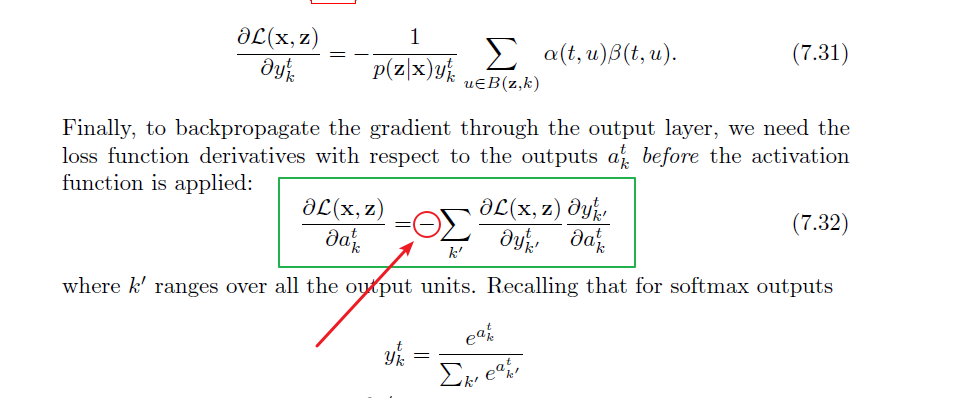
\includegraphics[width=0.7\textwidth]{ctc-wrong}
  \caption{原Alex博士论文中链式求导部分的错误 \label{fig:ctc-error}}
\end{figure}

\subsection{CTC的解码}
CTC的解码常用的有两种方式,greedy search和prefix beam search。greedy解码速度很快,但是很容易出错,但是prefix beam search解码速度慢,准确率较高。接下来挨个介绍两种解码方式的算法和流程,以及对应的代码解释。
\subsubsection{greedy search}
greedy search,也就是best path search,就是说找个每个时间点输出的最大概率值对应的标签,然后去重,再去掉blank。这种方式很快,因为不需要考虑整个路径输出,只考虑当前时刻的输出即可。。但是这种方式效果不太好,输出可能比较奇怪。代码如下,来自\upcite{greedy-search},这个库中还包含了一些关于CTC解码的论文。
\begin{lstlisting}[language = shell, numbers=left, 
         numberstyle=\tiny,keywordstyle=\color{blue!70},
         commentstyle=\color{red!50!green!50!blue!50},frame=shadowbox,
         rulesepcolor=\color{red!20!green!20!blue!20},basicstyle=\ttfamily]
def ctcBestPath(mat, classes):
  "implements best path decoding as shown by Graves (Dissertation, p63)"

  # dim0=t, dim1=c
  maxT, maxC = mat.shape  #blank的索引是最后一个
  label = ''  #初始化输出标签序列
  blankIdx = len(classes)  
  lastMaxIdx = maxC # init with invalid label

  for t in range(maxT):
    maxIdx = np.argmax(mat[t, :])  #找到当前帧最大标签的索引

    if maxIdx != lastMaxIdx and maxIdx != blankIdx:  #去重去blank
      label += classes[maxIdx]

    lastMaxIdx = maxIdx  #重置上一个标签的索引

  return label
\end{lstlisting}

\subsubsection{prefix beam search}
First-Pass Large Vocabulary Continuous Speech Recognition using Bi-Directional Recurrent DNNs\upcite{prefix-bs}中针对CTC提出了一种prefix beam search的算法,这种算法能够避免全局搜索的复杂度过高无法实现的问题,同时比greedy search的结果要好很多。

首先介绍下一些公式。公式\ref{eqn:with-lm}是最终的解码公式,配合语言模型和网络输出(声学模型),得到最有可能的$W$词序列。
\begin{align}
\label{eqn:with-lm}
W = \arg\mathop{\max}_{W}p_{net}(W;X)p_{lm}^{\alpha}(W)|W|^{\beta}
\end{align}
其中$p_{net}$是网络的输出,$p_{lm}$是语言模型的输出,$\alpha$和$\beta$分别为语言模型的权重和补偿系数。一般情况下,我们会降低语言模型对整体输出的影响,所以$\alpha$一般取$0.2$ ~ $0.7$。

接下来我们讲一下prefix beam search的demo\upcite{prefix-beam-search}。

总体是有三个循环,第一个是时间维度上的,时间$t$从$1$到$T$,也就是逐帧解码。第二个是对应候选输出序列的,这个是beam search,那么一定得设置一个beam size,那么会考虑所有的候选序列跟当前输出结合起来的概率值,那当前输出的话被剪枝之后还有很多个标签,再挨个的把每一个候选和每一个当前帧的标签进行结合计算。然后再利用这个结合的概率值进行重新排序得到新的候选。

\begin{lstlisting}[language = shell, numbers=left, 
         numberstyle=\tiny,keywordstyle=\color{blue!70},
         commentstyle=\color{red!50!green!50!blue!50},frame=shadowbox,
         rulesepcolor=\color{red!20!green!20!blue!20},basicstyle=\ttfamily]
pruned_alphabet = [alphabet[i] for i in np.where(ctc[t] > prune)[0]]
\end{lstlisting}

这一步是为了减少计算,也就是说先设定一个阈值,当前$t$时刻的时候,会做一个判断,只有当前时刻各个标签概率值大于 prune 的时候才会去做后续的操作,这就意味着当前时刻所有概率低于 prune 的标签都会被抛弃,不再参与到当前时刻的解码过程中。因为这些标签概率值太小,不太可能是正确的输出标签,留着只会增加计算量,还不如删掉,省时省心省力!

\begin{lstlisting}[language = shell, numbers=left, 
         numberstyle=\tiny,keywordstyle=\color{blue!70},
         commentstyle=\color{red!50!green!50!blue!50},frame=shadowbox,
         rulesepcolor=\color{red!20!green!20!blue!20},basicstyle=\ttfamily]
if len(l) > 0 and l[-1] == '>':
  Pb[t][l] = Pb[t - 1][l]
  Pnb[t][l] = Pnb[t - 1][l]
  continue 
\end{lstlisting}

这一步就是判断下是不是到结尾了,结尾的表示符号是">"。如果到了结尾呢,说明这个时候输出的标签序列和$t-1$时刻是一毛一样滴。$t$时刻输出序列$l$以 blank 结尾的概率跟$t-1$时刻以 blank 结尾的概率是一样的,$t$时刻输出序列$l$以 non-blank 结尾的概率跟$t-1$时刻以 non-blank 结尾的概率是一样的。然后就跳出当前时刻,因为当前时刻表示这个序列已经到了结尾了,没必要再折腾下去了。
 
\begin{lstlisting}[language = shell, numbers=left, 
         numberstyle=\tiny,keywordstyle=\color{blue!70},
         commentstyle=\color{red!50!green!50!blue!50},frame=shadowbox,
         rulesepcolor=\color{red!20!green!20!blue!20},basicstyle=\ttfamily]
if c == '%':
  Pb[t][l] += ctc[t][-1] * (Pb[t - 1][l] + Pnb[t - 1][l])
\end{lstlisting}

我们假设$\%$代表blank这个标签。剪枝之后,会对还剩下的那些标签走一遍遍历,每一个标签都会尝试着和之前存起来的候选序列进行结合,算出来一个概率值。那么既然是遍历,当然会轮到牛逼的 blank。所以首先看看当前的这个标签是不是blank。如果是blank的话,我们就没必要对当前的这个候选序列做啥子改动了,也就是当前时刻的输出标签序列还是$l$,因为最终输出的时候,blank也不会出现。既然当前这个标签是blank,那么$t$时刻的标签序列$l$的概率需要和当前时刻输出为 blank 的概率结合一下,变成当前时刻的 $Pb[t][l]$。其计算公式从代码里就可以看到。

\begin{lstlisting}[language = shell, numbers=left, 
         numberstyle=\tiny,keywordstyle=\color{blue!70},
         commentstyle=\color{red!50!green!50!blue!50},frame=shadowbox,
         rulesepcolor=\color{red!20!green!20!blue!20},basicstyle=\ttfamily]
l_plus = l + c
if len(l) > 0 and c == l[-1]:
  Pnb[t][l_plus] += ctc[t][c_ix] * Pb[t - 1][l]
  Pnb[t][l] += ctc[t][c_ix] * Pnb[t - 1][l]
\end{lstlisting}

如果说当前时刻的标签不是 blank,而是上个时刻的这个候选序列的最后一个输出标签,也就是说当前时刻的输出和上一个时刻的候选序列尾部产生了重复,这个时候其实是有两种情况的,第一种情况是上一个时刻的输出标签正好是 blank,因为从上面那一步代码中我们可以看出来,候选序列中是不会出现blank的,那如果是这种的情况,说明实际的输出序列就是有两个一样的字母,输出就是$l\_plus$,其尾部有两个一样的字母,这个时候候选序列的概率就等于当前时刻的标签概率乘以上一个时刻输出为blank的序列概率,也就是$Pb[t - 1][l]$;第二种情况是上一个时刻的输出确实也是这个标签,那么说明这个时候的候选序列不需要做啥变动,但是概率值需要变一下,当前时刻标签概率乘以上一个时刻输出是 non-blank 的序列概率值。

\begin{figure}[h]
  \centering
  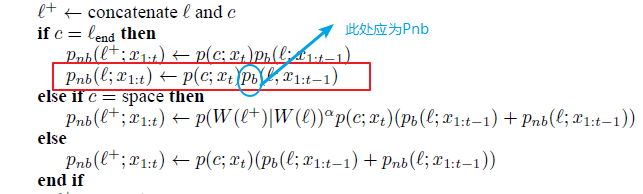
\includegraphics[width=0.6\textwidth]{error-prefix}
  \caption{Prefix Beam Search原论文中算法错误地方 \label{fig:error-prefix}}
\end{figure}

另外原论文中关于这一块的计算步骤写错了,也就是算法中的这一步,如图\ref{fig:error-prefix}。简直坑死个人。

\begin{lstlisting}[language = shell, numbers=left, 
         numberstyle=\tiny,keywordstyle=\color{blue!70},
         commentstyle=\color{red!50!green!50!blue!50},frame=shadowbox,
         rulesepcolor=\color{red!20!green!20!blue!20},basicstyle=\ttfamily]
elif len(l.replace(' ', '')) > 0 and c in (' ', '>'):
  lm_prob = lm(l_plus.strip(' >')) ** alpha
  Pnb[t][l_plus] += lm_prob * ctc[t][c_ix] * (Pb[t - 1][l] + Pnb[t - 1][l])
\end{lstlisting}

那还有可能当前的输出是 ' '(space),也就是说输出是空格或者是结尾,这个时候说明一个完整的词出现了,我们就可以利用语言模型(LM)来对输出进行修正和约束,避免出现毫无意义的结果。那么这个词代入到语言模型中会出现一个概率值,当前候选序列的概率值就通过公式\ref{eqn:with-lm}来计算,从代码中也可以看出来。

\begin{lstlisting}[language = shell, numbers=left, 
         numberstyle=\tiny,keywordstyle=\color{blue!70},
         commentstyle=\color{red!50!green!50!blue!50},frame=shadowbox,
         rulesepcolor=\color{red!20!green!20!blue!20},basicstyle=\ttfamily]
Pnb[t][l_plus] += ctc[t][c_ix] * (Pb[t - 1][l] + Pnb[t - 1][l])
\end{lstlisting}

还有最后一种情况,就是既不是 blank,又不是 space,当前输出标签和候选标签序列的最后一个字母也不一样,这个时候,就直接算出候选标签序列和当前标签的概率乘积就行,候选标签序列也有两种情况:上一个时刻以blank或者以non-blank结尾。综上集中基本的情况都已经讲完了。

\begin{lstlisting}[language = shell, numbers=left, 
         numberstyle=\tiny,keywordstyle=\color{blue!70},
         commentstyle=\color{red!50!green!50!blue!50},frame=shadowbox,
         rulesepcolor=\color{red!20!green!20!blue!20},basicstyle=\ttfamily]
if l_plus not in A_prev:
  Pb[t][l_plus] += ctc[t][-1] * (Pb[t - 1][l_plus] + Pnb[t - 1][l_plus])
  Pnb[t][l_plus] += ctc[t][c_ix] * Pnb[t - 1][l_plus]
\end{lstlisting}

按照原始论文中,还有上面这个公式。也就是说算出来的$l\_plus$不在候选标签序列里面,就会去之前时刻的候选序列里面去找,再利用之前的后续序列概率计算当前的概率值。百度的Deep Speech2代码里面说:这个部分不知道在干啥,还没啥用,所以就给去掉了。

我觉得……也不太好理解……

讲到这儿核心的代码部分已经讲完了,剩下的就是把当前时刻的标签,不管是以blank结尾的还是非blank结尾的综合起来,然后进行排序,根据beam size的大小得到新的候选序列,如此循环往复,直到这个序列输出到了尽头,就可以得到最终的结果啦\~\~\~

完整代码如下:

%%%%%%%%%%%%%%%%%%%%%%%Code for Prefix Beam Search%%%%%%%%%%%%%%%%%%%%%%%%%%%%%%%%%
\begin{lstlisting}[language = python, numbers=left, 
         numberstyle=\tiny,keywordstyle=\color{blue!70},
         commentstyle=\color{red!50!green!50!blue!50},frame=shadowbox,
         rulesepcolor=\color{red!20!green!20!blue!20},basicstyle=\ttfamily]
from collections import defaultdict, Counter
from string import ascii_lowercase
import re
import numpy as np

def prefix_beam_search(ctc, lm=None, k=25, alpha=0.30, beta=5, prune=0.001):
  """
  Performs prefix beam search on the output of a CTC network.

  Args:
    ctc (np.ndarray): The CTC output. Should be a 2D array (timesteps x alphabet_size)
    lm (func): Language model function. Should take as input a string and output a probability.
    k (int): The beam width. Will keep the 'k' most likely candidates at each timestep.
    alpha (float): The language model weight. Should usually be between 0 and 1.
    beta (float): The language model compensation term. The higher the 'alpha', the higher the 'beta'.
    prune (float): Only extend prefixes with chars with an emission probability higher than 'prune'.

  Retruns:
    string: The decoded CTC output.
  """

  lm = (lambda l: 1) if lm is None else lm # if no LM is provided, just set to function returning 1
  W = lambda l: re.findall(r'\w+[\s|>]', l)
  alphabet = list(ascii_lowercase) + [' ', '>', '%']
  F = ctc.shape[1]
  ctc = np.vstack((np.zeros(F), ctc)) # just add an imaginative zero'th step (will make indexing more intuitive)
  T = ctc.shape[0]

  # STEP 1: Initiliazation
  O = ''
  Pb, Pnb = defaultdict(Counter), defaultdict(Counter)
  Pb[0][O] = 1
  Pnb[0][O] = 0
  A_prev = [O]
  # END: STEP 1

  # STEP 2: Iterations and pruning
  for t in range(1, T):
    pruned_alphabet = [alphabet[i] for i in np.where(ctc[t] > prune)[0]]
    for l in A_prev:
      
      if len(l) > 0 and l[-1] == '>':
        Pb[t][l] = Pb[t - 1][l]
        Pnb[t][l] = Pnb[t - 1][l]
        continue  

      for c in pruned_alphabet:
        c_ix = alphabet.index(c)
        # END: STEP 2
        
        # STEP 3: “Extending” with a blank
        if c == '%':
          Pb[t][l] += ctc[t][-1] * (Pb[t - 1][l] + Pnb[t - 1][l])
        # END: STEP 3
        
        # STEP 4: Extending with the end character
        else:
          l_plus = l + c
          if len(l) > 0 and c == l[-1]:
            Pnb[t][l_plus] += ctc[t][c_ix] * Pb[t - 1][l]
            Pnb[t][l] += ctc[t][c_ix] * Pnb[t - 1][l]
        # END: STEP 4

          # STEP 5: Extending with any other non-blank character and LM constraints
          elif len(l.replace(' ', '')) > 0 and c in (' ', '>'):
            lm_prob = lm(l_plus.strip(' >')) ** alpha
            Pnb[t][l_plus] += lm_prob * ctc[t][c_ix] * (Pb[t - 1][l] + Pnb[t - 1][l])
          else:
            Pnb[t][l_plus] += ctc[t][c_ix] * (Pb[t - 1][l] + Pnb[t - 1][l])
          # END: STEP 5

          # STEP 6: Make use of discarded prefixes
          if l_plus not in A_prev:
            Pb[t][l_plus] += ctc[t][-1] * (Pb[t - 1][l_plus] + Pnb[t - 1][l_plus])
            Pnb[t][l_plus] += ctc[t][c_ix] * Pnb[t - 1][l_plus]
          # END: STEP 6

    # STEP 7: Select most probable prefixes
    A_next = Pb[t] + Pnb[t]
    sorter = lambda l: A_next[l] * (len(W(l)) + 1) ** beta
    A_prev = sorted(A_next, key=sorter, reverse=True)[:k]
    # END: STEP 7

  return A_prev[0].strip('>')

\end{lstlisting}

%------------------------------------------------------------------------------
%                                RNN Tranducer 
%------------------------------------------------------------------------------
\section{RNN-Tranducer}
RNN-Tranducer,简称RNN-T,同样是Alex Graves大神的作品\upcite{rnnt-1,rnnt-2}。
%------------------------------------------------------------------------------
%                                Attention 
%------------------------------------------------------------------------------
\section{Attention}

%------------------------------------------------------------------------------
%                                Transformer 
%------------------------------------------------------------------------------
\section{Transformer}


%------------------------------------------------------------------------------
%                                CNNs 
%------------------------------------------------------------------------------
\section{CNNs}

%------------------------------------------------------------------------------
%                                Mixed Models 
%------------------------------------------------------------------------------
\section{Mixed Models}

\subsection{Self-Attention Transducers for End-to-End Speech Recognition}
这篇论文的作者是田正坤,来自中国科学院自动化所。本论文的主要贡献有:
\begin{enumerate}
  \item 用self-attention模块替代了原来RNN-T中的RNN部分,可以用于并行计算;
  \item 利用 path-aware regularization 帮助SA-T学习对齐;
  \item 使用了chunk-flow机制来进行解码。
\end{enumerate}

\subsubsection{SA-T的基本结构}

\subsubsection{path-aware regularization}

\subsubsection{chunk flow mechanism}


\section{如何计算WER?}


\section{thinking about end-to-end speech recognition} 
\begin{enumerate}
  \item 只要在模型中用了卷积,卷积的stride如果比1大,或者no padding,那么就一定会造成时间轴上的压缩,如果时间轴上造成了压缩,最终softmax输出的标签序列和输入的特征序列的长度肯定是不一样的,输出的标签序列一定是比输入的要短,那就很难输出时间点(timestamp),也就是说我们是不知道每一帧输出的是啥玩意的……这个就很尴尬了,能不能加入点东西,用来记录缩短了之后的这个输出,每一个时间点对应着输入中的哪些时间点呢?

\end{enumerate}